\chapter{Odpowiedź skokowa obiektu rzeczywistego}

\begin{figure}[h!]
\centering
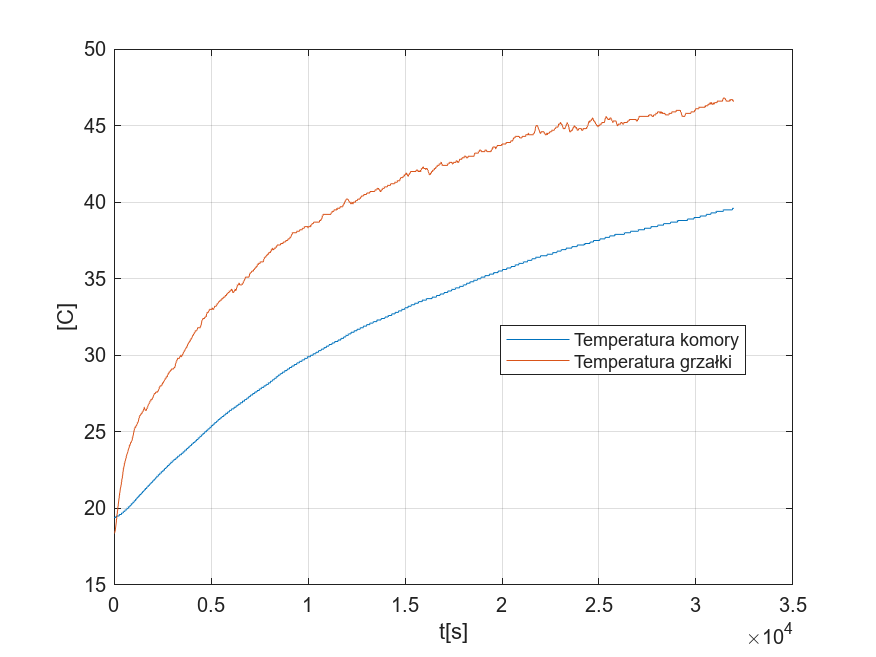
\includegraphics[width=\textwidth]{pictures/step_response}
\caption{Odpowiedź skokowa obiektu rzeczywistego.}
\label{step_response}
\end{figure}

Identyfikowanym obiektem była komora, która ogrzewana jest grzałką, która z kolei jest sterowana sygnałem PWM. Na Rys. \ref{step_response} przedstawiłem odpowiedź układu na wymuszenie w postaci $5\%$ wypełnienia sygnału PWM. Wymuszenie było tak małe ponieważ wcześniej wykonałem test na $10\%$ wymuszeniu i grzałka osiągnęła ok. $120^oC$ (dostałem pozwolenie na testowanie do $150^oC$), a na wykresie nie było widać wypłaszczenia temperatury, więc byłem zmuszony przerwać testy. Zastanawiam się jak rozwiązać ten problem, ponieważ steruję sygnałem PWM, a wejściem jest temperatura, jak skorelować ograniczenia temperaturowe z sygnałem PWM? Jednocześnie nie mogę ograniczyć sygnału sterującego w ramach +5, -5, bo regulator będzie bardzo wolny. Prosiłbym o wskazówki.

Postaram się ponowić testy, na mniejszej komorze, ponieważ obecnie testowana jest względnie duża i bardzo długo się nagrzewa i chłodzi (skończyłem testy o 21.00 i temperatura wskazywała ok. $40^oC$, rano zachodząc do pracy o 7.30 temperatura utrzymywała się na poziomie ok. $33^oC$).

\newpage

Zastanawiałem się również co w przypadku gdyby obiekt rzeczywisty był jednak liniowy. Na przedmiocie TAP realizowaliśmy projekt, którego tematem był obiekt MISO o silnych nieliniowościach.

\begin{figure}[h!]
\centering
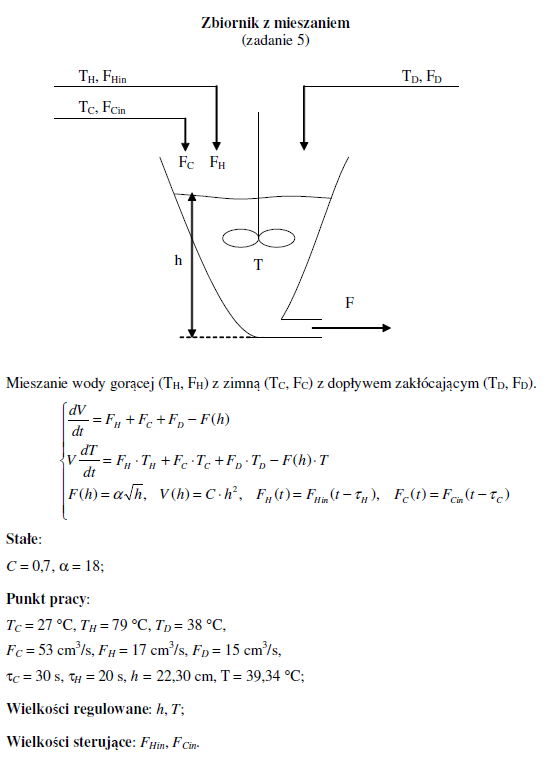
\includegraphics[width=0.9\textwidth]{pictures/zadanie_tap}
\caption{Obiekt MISO.}
\end{figure}

\textbf{Czy w razie gdyby obiekt rzeczywisty okazał się liniowy, jako alternatywa mógłbym zamodelować obiekt z zadania czy jednak wybierzemy jeszcze bardziej złożony?}s